\section{Measurements}

During the first section we have introduced the concept of measure as a set $\{ \hat{\Pi}_n \}_{n\in\mathcal{I}}$ of operators that allow us to evaluate the probability of having a certain outcome $\lambda_n$ for the measure of a physical quantity $\Lambda$. Nevertheless, even if we have listed the main properties that such operators should have we didn't specify the forms that they can possess. It is now time to introduce the main way in which such set of operators can present themselves and how they will work inside quantum circuits.

\subsection{Projection valued measurement}

If we take a look back to the different properties stated in Def. (\ref{def:measure}) an idea should arise, especially by looking at the collapse condition. The latter, in fact, can be thought as the state of the system gets projected into a certain state that posses a definite value of the physical quantity we are interested in measuring. In fact, it's easy to see how the following is true
\begin{align}
    &\hat{\Pi}_n \ket{\psi_n} = \ket{\psi_n}, &p_n = \ev{\hat{\Pi}_n^\dagger\hat{\Pi}_n}{\psi_n} = 1.
\end{align}
Operators that posses this effect of taking a general state $\ket{\psi}$ and taking it into another are really known in mathematics and are called \textbf{projector operators}, represented as $\hat{P}$. This type of operator is defined, in particular, by two main conditions
\begin{align}
    \label{eq:ProjDef}
    &\hat{P}^\dagger = \hat{P}, & \hat{P}^2 = \hat{P},
\end{align}
these two properties are enough to give $\hat{P}$ a lot of power allowing it to define alone a subspace of the vector space in which is working. In our case this means
\begin{equation}
    \mathcal{P} = \left\{ \left.\ket{\psi}\right| \exists \ket{\phi} \in \mathcal{H}: \ket{\psi} = \hat{P}\ket{\phi} \right\},
\end{equation}
basically we are aiming to create a set $\{ \hat{P}_n \}$ so that $\mathcal{P}_n$ is the eigenspace of $\lambda_n$. Therefore, it's easy to understand that on a general ground we are searching for a specific type of measure constructed using projectors, that will take the following specific name and definition.
\dfn{Projection valued measurement}
{
    We will call projection valued measurement, or PVM, a set of operators $\{ \hat{P}_n \}_{n\in\mathcal{I}}$ so that $\hat{P}_n$ is a projector and the whole set is a measure.
}

To find out the right projectors to create the complete set we can simply use the properties of the observable in QM. An observable quantity is represented in QM using an operator $\hat{\Lambda}$ and the possible values that $\Lambda$ can take, the outcomes, are the eigenvalues of that operator $\lambda_n$. Nevertheless, for a general operator $\lambda_n$ can be complex, or worst they can not exist, that is a problem since is absurd to mesure a complex number in an experiment, therefore we will make a further assumption giving out the following definition.
\dfn{Observables}
{
    An observable $\Lambda$ in QM is represented by a hermitian operator $\hat{\Lambda}$, so that
    \begin{equation}
        \hat{\Lambda}^\dagger = \hat{\Lambda}.
    \end{equation}
}
\noindent
A really important theorem of linear algebra called \textbf{spectral theorem} allow us to say that, with this further assumption of hermiticy, the operator can be diagonalyzed and the eigenvalues are all real. Along with that, the spectral theorem also allow us to say that a set of eigenstates $\{\ket{\psi_n}\}$ with the following properties exist
\begin{equation}
    \label{eq:BaseDef}
    \hat{\Lambda}\ket{\psi_n} = \lambda_n\ket{\psi_n}, \hspace{2cm} \braket{\psi_n}{\psi_m} = \delta_{nm}, \hspace{2cm} \sum_n \ketbra{\psi_n}{\psi_n} = \mathbb{1},
\end{equation}
forming an orthonormal base for $\mathcal{H}$. These properties should hint us that the set of projectors that we want to create to measure $\Lambda$ may be the ones that project onto the eigenspace generated by $\ket{\psi_n}$, and we can easily see how that is the case. 

\thm{Observable PVM}
{
    Taken $\hat{\Lambda}$ an observable the set of projectors $\{ \hat{P}_n \}_{n\in\mathcal{I}}$ onto the orthonormal base of eigenstate $\{\ket{\psi_n}\}_{n\in\mathcal{I}}$ of $\hat{\Lambda}$ forms a measure for the observable itself called \textbf{Projection valued measurement}.
}
\pf{Proof}
{
    We are going to define the projector $\hat{P}_n$ as follows
    \begin{equation}
        \hat{P}_n = \ketbra{\psi_n},
    \end{equation}
    which can be easily seen it's a projector, the demonstration is left to the reader. We want to see how all the requirement in Def. (\ref{def:measure}) are verified, we can start from the probability by taking a general state $\ket{\psi}$ and writing
    \begin{align}
        &\ket{\psi} = \sum_n c_n\ket{\psi_n},   & p_n = \ev{\hat{P}^\dagger_n\hat{P}_n}{\psi} = \ev{\hat{P}_n}{\psi} = \abs{c_n}^2.
    \end{align}
    Where I have first written the expansion of $\ket{\psi}$ on the orthonormal base and then used the properties in \eqref{eq:ProjDef} and \eqref{eq:BaseDef} to obtain the probability. It's possible to see how the values of $\abs{c_n}^2$ effectively represents probabilities since also the condition \eqref{eq:MeasureCompleteCondition} is respected by the set of operators defined thanks to the completeness condition of the orthonormal base
    \begin{equation}
        \sum_n \hat{P}^\dagger_n\hat{P}_n = \sum_n \hat{P}_n = \sum_n \ketbra{\psi_n} = \mathbb{1}.
    \end{equation}
    Therefore, the first condition for having a measure is respected. We can now see how also the second one is obtained as we want since we can write
    \begin{equation}
        \ket{\psi_n} = \frac{\hat{P}\ket{\psi}}{\sqrt{\ev{\hat{P}^\dagger_n\hat{P}_n}{\psi}}} = \frac{c_n}{\sqrt{\abs{c_n}^2}}\ket{\psi_n} = e^{i\theta}\ket{\psi_n},
    \end{equation}
    and since a complex phase doesn't change the physical state of the system the wanted result is achieved.
}

\ex{Qubit PVM}
{
    To make an example we can use a qubit, where we can imagine measuring the state as $\ket{1}$ or $\ket{0}$, so a computational base measurament. We can also easily imagine what is the form of the operator, the observable, that has them as eigenstates
    \begin{align}
        &Z = \begin{pmatrix}
            1 & 0\\
            0 & -1
        \end{pmatrix}, &Z\ket{i} = \lambda_i\ket{i},
    \end{align}
    where it's easy to see, by using the $\mathbb{C}^2$ representation of the states, how $\lambda_0 = 1$ and $\lambda_1 = -1$. This means that for every state $\ket{\psi}$ we can measure the probability of a certain outcome, state $\ket{1}$ or $\ket{0}$, to appear by using the set of operators defined by $\hat{P}_i = \ketbra{i}$ given as matrix by
    \begin{align}
        &P_0 = \begin{pmatrix}
            1 & 0\\
            0 & 0
        \end{pmatrix},
        &P_1 = \begin{pmatrix}
            0 & 0\\
            0 & 1
        \end{pmatrix}.
    \end{align}
    Applied to a general vector they will give in general the first or second component, respectively.
}

\subsection{Positive operator valued measurement}

In the PVM description of measure that we have given just now we use projector operators to predict the probabilities, which posses a series of properties that makes them really well suited for the task. Nevertheless, they are not the only possible choice, in particular such projectors posses the property of being hermitian that general measures can totally not have. We want so to see a case where another type of measure respect to the PVM can be a better choice to study the system.

Let's imagine having a qubit and a quantum circuit that is able to prepare it in two states given by
\begin{align}
    &\ket{\psi_1} = \ket{0}, & \ket{\psi_2} = \frac{\ket{0} + \ket{1}}{\sqrt{2}}.
\end{align}
We want to see if we are able to understand which state after a measure. Using the PVM measure of a qubit using $Z$ as an observable we can easily see how $\ket{\psi_1}$ posses a probability equal to $1$ of being in state $\ket{0}$, while $\ket{\psi_2}$ has $p_i = 1/2$ for both states. This means that if I take a measure and the outcome is $\lambda = -1$ I know that the only state that can have that outcome is $\ket{\psi_2}$ since has a non-zero probability of being in state $\ket{1}$. Instead, if the result is $\lambda = 1$ I can't say which one of the two state is the right one. We can also understand why we are not able to decide, since the two states that we are working with are not orthogonal respect to the computational base and so $\ket{\psi_2}$ has non-zero probability of being in both states. Therefore, we would like to use a set of operators that instead are able to give us this property, and a possible way of obtaining them is by taking $\{ \hat{\Pi}_n \}$ so that
\begin{equation}
    \hat{\Pi}_n^\dagger\hat{\Pi}_n = \hat{E}_n,
\end{equation}
are \textbf{positive valued operators}. In this way we are allowed to define as our operators the following objects
\begin{align}
    &\hat{E}_1 = \ketbra{1}, &\hat{E}_2 = \left( \frac{\ket{0} - \ket{1}}{\sqrt{2}} \right)\left( \frac{\bra{0} - \bra{1}}{\sqrt{2}} \right),
\end{align}
basically the projector on the states that are orthogonal to the ones that we were looking at. Nevertheless, the set composed by $\hat{E_1}$ and $\hat{E}_2$ is not sad to respect the relation \eqref{eq:MeasureCompleteCondition} meaning that we are needed to add a third element in general that allow for the set to be a measure
\begin{equation}
    \hat{E}_3 = \mathbb{1} - \hat{E}_2 - \hat{E}_1.
\end{equation}
Then, using this new set we are able to obtain a more satisfying result since the now the possible outcomes of the measurement are three. In fact, we can imagine that doing a measure using $\{\hat{E}_n\}$ is experimentally equivalent to obtain three possible outcomes $\lambda_n$ where the probabilities of the outcomes for the two states respectively are
\begin{align}
    &\ev{\hat{E}_i}{\psi_1} = \begin{cases}
        p_1 = 0\\
        p_2 \neq 0\\
        p_3 \neq 0
    \end{cases},
    &\ev{\hat{E}_i}{\psi_2} = \begin{cases}
        p_1 \neq 0\\
        p_2 = 0\\
        p_3 \neq 0
    \end{cases}.
\end{align}
Therefore, now after a measure we are able to say that if the outcome is $\lambda_1$ or $\lambda_2$ the result is state $\ket{\psi_1}$ or $\ket{\psi_2}$ respectively, while $\lambda_3$ is telling us that the measure is not satisfying since we can't distinguish the two states. This may seem not so different respect to the PVM measure since still we have the case where the single measure can distinguish the two cases, but here we have also an outcome that tells us with certainty to have $\ket{\psi_2}$ that we didn't have before. Also, it is possible to demonstrate that the probability of an not satisfying measure is minimized by this set.

Therefore, with this simple case we have seen how the definition of measure in reality leaves large freedom in the choice of the operator set and not only projectors. In fact, we can now generaly define also the positive operator valued measurement as follows.
\dfn{POVM}
{
    We will call positive operator valued measurement a set of operators $\{ \hat{E}_n \}_{n\in\mathcal{I}}$ so that $\hat{E}_n$ is a positive valued operator and the whole set represent a measure.
}
\noindent
This definition is much more general than PVM and can allow for better result in terms of computations as we have seen in the example shown beforehand. Nevertheless, the problem of these measures is that we actually don't know how to represent them in practice. In fact, for PVM the definition was made starting from a physical observable while here the physical representation is much more hidden. Still, doesn't mean that don't exist. Is possible to demonstrate that whatever measure, can be represented into a higher dimensional space through a unitary transformation composed a PVM, in this way everything can be physically interpreted. We can so state the following result in terms related to quantum computers applications as follows.
\thm{Representation of measures}
{
    Any generalized measure on a system of $N$ qubit $\mathcal{H}_Q$ can be realized as a PVM with the aid of auxiliary qubit and a unitary operator.
}
\pf{Proof}
{
    Imagine having a general measure $\{ \hat{\Pi}_n \}_{n\in\mathcal{I}}$ acting on $\mathcal{H}_Q$, we can take an orthonormal set $\{ \ket{m} \}_{m\in\mathcal{I}'}$, with $\#\mathcal{I} = \#\mathcal{I}'$, of states $\ket{m}\in \mathcal{H}_Q$ and construct an auxiliary space as
    \begin{align}
        &\mathcal{H}_{tot} = \mathcal{H}_Q\otimes \mathcal{H}_M, &\mathcal{H}_M = \text{span}\{\ket{m}\}.
    \end{align}
    So, a general state inside the auxiliary space can be written as $\ket{\psi}\ket{s}$, with $\ket{\psi}\in \mathcal{H}_Q$ and $\ket{s}\in\mathcal{H}_M$. Now, we define the transformation $\mathcal{U}$ as follows
    \begin{equation}
        \mathcal{U}\ket{\psi}\ket{s} = \sum_n \left( \hat{\Pi}_n\ket{\psi} \right)\ket{m},
    \end{equation}
    which can be seen to be a unitary operator since the following relation can be obtained
    \begin{equation}
        \bra{s}\bra{\psi}\mathcal{U}^\dagger\mathcal{U}\ket{\phi}\ket{s} = \sum_{mm'}\mel{\psi}{\hat{\Pi}_{m'}^\dagger\hat{\Pi}_m}{\phi}\braket{m'}{m} = \sum_m \mel{\psi}{\hat{\Pi}_{m}^\dagger\hat{\Pi}_m}{\phi} = \braket{\psi}{\phi}.
    \end{equation}
    Where the relation $\braket{m}{m'} = \delta_{mm'}$ and $\sum_n \hat{\Pi}_{m'}^\dagger\hat{\Pi}_m = \mathbb{1}$ have been used during the process, demonstrating that $\mathcal{U}$ conserve the norm of the space being so unitary. Next we can define the projection operators to be given by the following
    \begin{equation}
        \hat{P}_m = \mathbb{1}_Q \otimes \ketbra{m},
    \end{equation}
    creating a PVM set of measure. Then, we can see how the operator $\hat{P}_m\mathcal{U}$ act on a general state of the whole space as
    \begin{equation}
        \hat{P}_m\mathcal{U}\ket{\psi}\ket{s} = \sum_{m'} \left( \hat{\Pi}_n\ket{\psi} \right)\braket{m}{m'} \ket{m}= \hat{\Pi}_m\ket{\psi}\ket{m}.
    \end{equation}
    This is a powerful result since we can already see how this set of operations is able to reproduce the general measure in all of it's fascion. We can start by seeing how the probabilities that predicts are the same
    \begin{equation}
        p_m = \bra{s}\bra{\psi}\mathcal{U}^\dagger\hat{P}_m^\dagger\hat{P}_m\mathcal{U}\ket{\psi}\ket{s} = \ev{\hat{\Pi}_n^\dagger\hat{\Pi}_n}{\psi}.
    \end{equation}
    Thus, also the projection remains unchanged under the effect of this operator since
    \begin{equation}
        \frac{\hat{P}_m\mathcal{U}\ket{\psi}\ket{s}}{\sqrt{\bra{s}\bra{\psi}\mathcal{U}^\dagger\hat{P}_m^\dagger\hat{P}_m\mathcal{U}\ket{\psi}\ket{s}}} = \frac{\hat{\Pi}_m\ket{\psi}}{\sqrt{\ev{\hat{\Pi}_n^\dagger\hat{\Pi}_n}{\psi}}}\ket{m} = \ket{\psi_m}\ket{m}.
    \end{equation}
    Therefore, all the properties of the general measure are conserved, meaning that $\{ \hat{P}_m\mathcal{U} \}$ successfully represent it.
}
\noindent
This result is telling is that doesn't matter with measure we are using we can always add a number of qubit so that the space becomes larger by a $\mathcal{H}_M$ with dimensions equal to the number of outcomes you want to measure and use a normal PVM along with a unitary transformation defined by the measure itself. In this way we can always use the same $Z$ gate seen in the PVM example to measure the auxiliary qubit and based on the value of their state, which gives $\ket{m}$, we can know the outcomes of the others, since $\ket{m}$ correspond to a collapsed $\ket{\psi_m}$ and so $\lambda_m$ as outcome.

\nt
{
    This whole theory was though first by Von Neumann which tried to create it to describe the collapse on the wavefunction in a rigorous way. In particular He though that an experimental apparatus in general was the auxiliary system $\mathcal{H}_M$ that taking the measure made the system collapse in the way we have seen.
}

\subsection{Measurements and circuits}

Measuring is an important feature inside a quantum circuits since at the end of the manipulations we also need to know the result of the operations contained in the qubits states. In general, we are going to see how the measurement works inside a quantum circuit and their properties. First, we shall keep in mind that usually all the quantum computers are able to perform measurements mainly in the computational basis, meaning of the observable $Z$. This is due to a matter of experimental convenience, but lead us to try to reconduce every possible measure to that one. For example, we may work for a complex quantum circuit in a base like $\ket{\pm}$ so that a state is given by
\begin{equation}
    \ket{\psi} = a\ket{+} + b\ket{-},
\end{equation}
but we can't use the measure given in that base since the QC only measure in computational base. The answer to this problem is in reality incredibly simple, and we can state it really quickly as
\thm{Base change}
{
    Let's imagine having a circuit that prepare a qubit state $\ket{\psi}$ described on an orthonormal base $\ket{e_1}$ and $\ket{e_2}$. The measurement of the state can be performed still on the computational base without losing information by applying an appropriate rotation before the measure.
}
\pf{Proof}
{
    Let $\mathcal{U}$ be the unitary transformation that acts as follows
    \begin{align}
        &\mathcal{U}\ket{e_1} = \ket{0}, &\mathcal{U}\ket{e_2} = \ket{1},
    \end{align}
    we can easily see how the state $\ket{\psi}$ can be written in a really simple way by using the following reasoning
    \begin{equation}
        \ket{\psi} = a\ket{e_1} + b\ket{e_2} = \mathcal{U}\left( a\ket{0} + b\ket{1} \right).
    \end{equation}
    Meaning that the state $\mathcal{U}^\dagger\ket{\psi}$ will be a state written in the computational base with the same coefficients, therefore measuring it gives out the same probabilities of before we don't lose any informations.
}
\noindent
This little result is really helpful in practice, since basically means that we can perform a measurament using the same base in every possible situation by using circuit like in \figref{fig:Measure}.
\begin{figure}[b]
    \centering
    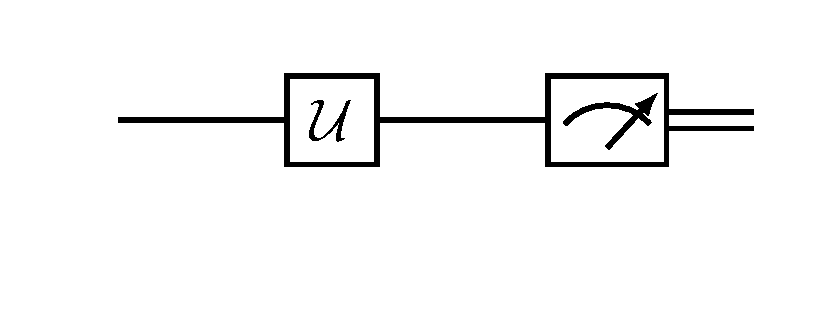
\includegraphics[width=0.8\textwidth]{Immagini/Measure.pdf}
    \caption{Simple quantum circuit for the measure of a qubit in a general base, composed by a rotation and the measure.}
    \label{fig:Measure}
\end{figure}
Where we can see how the measure is represented by the symbol with the arrow which take a quantum state and returns the outcome of the measure on a classical bit $1$ or $0$, seen as the double line.

% TODO: Qua devi fare l'esempio di come si misura uno stato anche se è descritto in termini di un'altra base facendo le rotazioni, qui ci può stare un disegno in modo tare da introdurre la notazione che non sarebbe affatto male, anche per la notazione del bit classico.

% TODO: Devi metterci il principio del "lo puoi mettere dove cazzo ti pare" e del "misura implicita"

% TODO: Controllo classico o controllo quantistico, ma lo puoi infilare anche dentro al principio del, lo puoi mettere dove cazzo ti pare("anzi, fai l'esempio con quello così te lo levi subito")

The other important thing that we can say about measure inside circuits is that they can be applied in every point of the circuit and the final result of the computation will not change. To understand this we shall make an example using control gates as depicted in \figref{fig:ControlEquivalence}.
\begin{figure}[t]
    \centering
    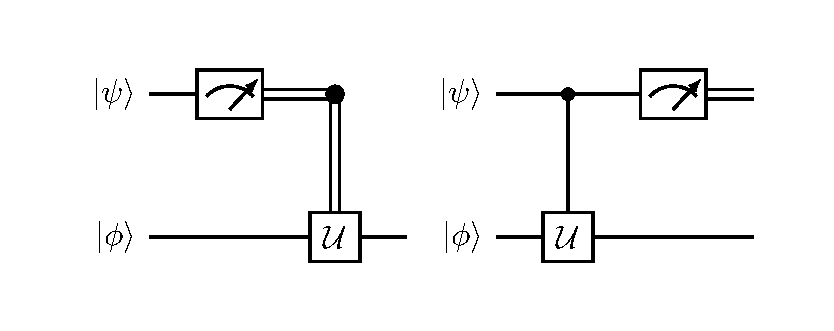
\includegraphics[width=\textwidth]{Immagini/ControlEquivalence.pdf}
    \caption
    {
        Representation of two equivalent circuits that uses classical and quantum control to apply an operation to the second qubit. In the first case the measurement on the first qubit is done before the control while in the other is done after, still the result will not change having that if the bit is $1$ the operation is applied, while if is $0$ will remain untouched.
    }
    \label{fig:ControlEquivalence}
\end{figure}
We can see how the two circuits differ based on where the measurement is placed in the circuit. Nevertheless, if we analyze the system we can simply see how the outcome of the state $\ket{\phi}$ will be the same based on the value of the measurement. In fact, take the first circuit: the outcomes were
\begin{equation}
    \ket{\phi}, \hspace{0.5cm} \text{if }c=1; \hspace{2cm} \mathcal{U}\ket{\phi}, \hspace{0.5cm} \text{if }c=0,
\end{equation}
where $c$ represent the value of the bit. Now, if we take the second one, it's easy to see that if the measure gives $1$ meant that the that $\ket{\psi}$ had a component along $\ket{1}$ passing through the control so that the rotation was applied to $\ket{\phi}$. Instead, if the value was $0$ the opposite happens having so that the outcome at the end will be the exact same. This property of measurement takes the name of \textbf{principle of deferred measurement}, and allow us to place the measurement procedure always at the end of our circuits without the worries of modifying the outcome of the algorithm.
\wc{Attention}
{
    The deferred measurement principle it's not based on a mathematical result, since for it work in a general case we shall need that the measure operator $\hat{\Pi}_m$ commute with every possible gate $\mathcal{U}$. In this way we would have that
    \begin{equation}
        \hat{\Pi}_m\mathcal{U}\ket{\psi} = \mathcal{U}\hat{\Pi}_m \ket{\psi},
    \end{equation}
    which means that the final state at the end of the circuit remains the same. Nevertheless, it's easy to find a counter example by using $\mathcal{U} = X$ and $\hat{\Pi}_m = \ketbra{1}$, meaning that in general may exist a situation where the final outcome changes. Still, the principle could still hold since our aim is not really find out the exact value of the final state, but to understand it by using a single measure and the connection between the probabilities of certain outcomes and possible prepared states. Therefore, even if mathematically the result can be different physically specking the result is the same.
}

\nt
{
    It's possible to find that in several circuits the final measures are not explicitly written or are written only on certain qubit, that is because only the necessary measurements to understand the states of the qubits are shown, the non-necessary ones are skipped. This idea is also called \textbf{principle of implicit measurements} and will be more clear as we will talk about entanglement.
}